\documentclass[conference]{IEEEtran}
\usepackage[utf8]{inputenc}
\usepackage[T1]{fontenc}
\usepackage{amsmath,amssymb}
\usepackage{graphicx}
\usepackage{booktabs}
\usepackage{listings}
\usepackage{xcolor}
\usepackage{hyperref}
\usepackage{cite}
\hypersetup{colorlinks=true,linkcolor=black,citecolor=black,urlcolor=blue}
\lstset{basicstyle=\ttfamily\scriptsize,breaklines=true,frame=single,columns=fullflexible,
        commentstyle=\color{gray},keywordstyle=\bfseries,language=C++}

\title{A Bitboard Chess Engine with Alpha--Beta Search, Transposition Table\\
       and Time-Budgeted Difficulty Levels in the natID Framework}

\author{\IEEEauthorblockN{Faris Muratovi\'c}
\IEEEauthorblockA{Project Report (Artificial Intelligence)\\
Student ID: 19958\\
Faculty of Electrical Engineering, University of Sarajevo\\
Instructor: Prof.\ Dr.\ Izudin D\v{z}afi\'c}}

\begin{document}
\maketitle

\begin{abstract}
This project is a complete chess application: a rules-exact game engine, an adversarial-search opponent, and a graphical front end built with the natID framework. The board is represented by twelve 64-bit bitboards, move generation is fully legal (castling, en passant, promotion, check and pin handling), and its correctness is established by perft: the node counts of four standard test positions agree with the published reference values up to 4.9~million leaves. The opponent searches the game tree with negamax and alpha--beta pruning, extended by quiescence search, a Zobrist-keyed transposition table, MVV--LVA capture ordering, killer and history heuristics, iterative deepening, mate-distance scoring and a root-parallel final iteration. Its evaluation combines material, tapered piece-square tables, bishop pair, pawn structure (doubled, isolated, passed), mobility, rook files and king shelter. Four difficulty levels are defined as time budgets per move (150~ms to 2.2~s) rather than fixed depths, so the response time is consistent across openings and endgames. The GUI offers human-versus-human and human-versus-bot play with drag-and-drop, legal-move highlighting, a promotion picker, undo/redo, captured-piece panels and two interface languages; the search runs on a worker thread so the interface never freezes. Measured on a single core the engine generates 11--17~million perft nodes per second and reaches depth~6 from the start position in 0.23~s.
\end{abstract}

\begin{IEEEkeywords}
chess, adversarial search, minimax, alpha--beta pruning, negamax, transposition table, Zobrist hashing, quiescence search, iterative deepening, bitboards, perft, natID
\end{IEEEkeywords}

\section{Introduction}
Chess is the canonical benchmark for adversarial search. It has a branching factor of roughly 35, a game tree far beyond exhaustive enumeration, perfectly defined rules, and a long history of published test positions against which an implementation can be checked exactly. Building a playable engine therefore exercises the whole of the classical AI search toolkit: minimax and alpha--beta pruning, move ordering, memoisation of the game tree, evaluation-function design, and the engineering that makes those algorithms fast enough to be useful under a clock.

The project delivers a desktop application with three layers. The \emph{engine} (\texttt{ChessBoard}) owns the position, generates legal moves and searches. The \emph{game controller} (\texttt{Chess} in \texttt{Connection.h}) maintains the game state, move history, draw rules and the human/bot turn logic, and drives the search on a background thread. The \emph{user interface} (\texttt{StartWindow}, \texttt{MainWindow}, \texttt{mainView}, \texttt{ViewSettings}) is written against natID's \texttt{natGUI} library and renders the board, pieces and panels on a canvas. The engine has no dependency on the GUI, which made it possible to verify it by compiling it stand-alone and running perft and search benchmarks from the command line; every number in Section~\ref{sec:results} was obtained that way.

\section{Background}
\subsection{Minimax, negamax and alpha--beta}
A two-player zero-sum game is solved by minimax: the value of a position is the maximum over the mover's options of the negated value of the resulting position for the opponent. Writing the recursion in this negated form (negamax) removes the distinction between maximising and minimising nodes. Alpha--beta pruning \cite{knuth} maintains a window $(\alpha,\beta)$ of scores that can still affect the root decision; a move that proves the position is worth at least $\beta$ for the mover causes a \emph{cutoff} because the opponent will never allow it. With perfect move ordering alpha--beta visits about $b^{d/2}$ nodes instead of $b^d$, so good ordering doubles the reachable depth for the same effort.

\subsection{Horizon effect and quiescence}
Stopping the search at a fixed depth and evaluating statically is misleading when the last move was a capture whose recapture lies just beyond the horizon. Quiescence search continues the search with captures only until the position is ``quiet'', bounding the extra work with a \emph{stand-pat} score.

\subsection{Transposition tables}
Different move orders frequently reach the same position. A transposition table memoises the score already computed for a position, keyed by a 64-bit Zobrist hash \cite{zobrist}: every (piece, square) pair, castling right, en-passant file and side to move has a random key, and the position's hash is the XOR of the keys of its features. Because XOR is its own inverse, a move updates the hash incrementally in a handful of operations.

\subsection{Bitboards}
A bitboard is a 64-bit integer with one bit per square \cite{cpw}. Keeping one bitboard per piece type and colour turns most questions about a position (``which white pieces attack square $s$?'') into a few AND/OR/shift operations and a population count, which is why every strong engine uses them.

\section{Board Representation}
\texttt{ChessBoard} holds twelve bitboards (\texttt{whitePawns} \ldots\ \texttt{blackKing}), the side to move, castling rights, the en-passant square, the half-move clock, and the incrementally maintained Zobrist hash. Population count and least-significant-bit extraction use \texttt{\_\_builtin\_popcountll} / \texttt{\_\_builtin\_ctzll} on GCC and Clang and the equivalent \texttt{<intrin.h>} functions on MSVC, chosen at compile time. Knight and king attack sets are precomputed tables; sliding attacks (bishop, rook, queen) are generated by ray walking, which is simpler than magic bitboards and, at the search depths used here, fast enough (Section~\ref{sec:results}).

A move is a compact \texttt{MoveBB} record: from-square, to-square, moving piece, captured piece, promotion piece, and flags for castling and en passant, plus the castling-rights and en-passant state before the move so that \texttt{undoMoveBB} can restore it exactly. \texttt{makeMoveBB} updates the bitboards, the rights and the hash in one pass; \texttt{undoMoveBB} recomputes the same hash delta and XORs it out. Positions can be loaded from FEN strings, which is how the test positions of Section~\ref{sec:results} are set up.

\section{Move Generation and Legality}
\texttt{getAllMovesBB} generates pseudo-legal moves for the side to move: pawn pushes (single and double), captures, en passant and the four promotion pieces, knight and king moves from the attack tables, sliding moves by ray walking, and castling when the king and rook have not moved, the squares between them are empty and the king does not pass through check. \texttt{getLegalMovesBB} then plays each move, tests \texttt{isKingInCheckBB} and unplays it, keeping only the moves that leave the mover's king safe. This make/unmake legality filter is simpler than pin detection and is exact by construction.

The generator's correctness is established by \emph{perft} (Section~\ref{sec:perft}), which counts every leaf of the legal game tree to a given depth; a single missing or spurious move changes the count. The engine passes all four standard positions, including Kiwipete, whose purpose is to exercise castling, promotion, en passant and pinned pieces simultaneously. Two generator bugs were found and fixed by perft during development (a rook-move omission and a hash desynchronisation), which is exactly the role the test is meant to play.

\section{Search}
\subsection{Negamax with alpha--beta and quiescence}
Listing~\ref{lst:negamax} shows the core of \texttt{negamaxBB}. Before anything else the transposition table is probed; a hit with sufficient depth and a compatible bound returns immediately. Positions that are drawn by rule (50-move, repetition, insufficient material) score 0 at any ply below the root. At depth 0 the search hands over to \texttt{quiescenceBB}, which searches captures only, with a stand-pat lower bound and a hard cap of eight extra plies. A position with no legal moves is checkmate if the king is in check and stalemate otherwise; the two are scored $-(\mathrm{MATE}-\mathrm{ply})$ and 0 respectively. Encoding the distance to mate in the score makes the engine prefer the shortest mate and avoid shuffling when it has a won position.

\begin{lstlisting}[caption={Negamax with alpha--beta, transposition table and quiescence (abridged from \texttt{ChessBoard.cpp}).},label=lst:negamax]
int ChessBoard::negamaxBB(int depth, int alpha, int beta,
        bool white, TranspositionTable& tt,
        SearchHeuristics& heur, int ply)
{
    nodeCount++;
    int ttScore;
    if (tt.probe(zobristHash, depth, alpha, beta, ttScore))
        return ttScore;
    if (ply > 0 && isDrawByRule()) return 0;
    if (depth == 0)
        return storeAndReturn(quiescenceBB(alpha, beta, white, 8));

    auto moves = getLegalMovesBB(white);
    if (moves.empty())                     // mate or stalemate
        return isKingInCheckBB(white) ? -MATE_SCORE + ply : 0;

    orderMovesWithHeuristics(moves, heur, ply);
    int best = -INF, alphaOrig = alpha;
    for (const auto& m : moves) {
        makeMoveBB(m);
        int s = -negamaxBB(depth-1, -beta, -alpha, !white, tt, heur, ply+1);
        undoMoveBB(m);
        best = std::max(best, s);  alpha = std::max(alpha, s);
        if (alpha >= beta) {                // beta cutoff
            if (m.captured == EMPTY && !m.promotion) {
                heur.recordKiller(ply, m);
                heur.recordHistory(m, depth);
            }
            break;
        }
    }
    tt.store(zobristHash, depth, best, boundFlag(best, alphaOrig, beta));
    return best;
}
\end{lstlisting}

\subsection{Transposition table}
\texttt{TranspositionTable} is a power-of-two array of entries (16~MB by default, indexed by a bit mask of the hash) storing key, depth, score and a flag \texttt{EXACT}, \texttt{LOWERBOUND} or \texttt{UPPERBOUND}. A probe succeeds only if the stored depth is at least the requested depth and the bound is usable for the current window: an exact score always, a lower bound only if it is $\ge\beta$, an upper bound only if it is $\le\alpha$. Every search node stores its result with the flag derived from how the final score relates to the original window.

\subsection{Move ordering}
Cutoffs come early only if good moves are tried first. Captures are scored by MVV--LVA (ten times the victim's value minus the attacker's value), promotions receive a large bonus, and quiet moves are ordered by two adaptive heuristics: \emph{killer moves} (the last two quiet moves that produced a cutoff at the same ply, tried first among quiets) and a \emph{history table} indexed by from/to square, incremented by the depth at which a move caused a cutoff and used as a tie-breaker.

\subsection{Iterative deepening and time control}
\texttt{findBestMoveBB\_ID} searches to depth 1, 2, \ldots, $d_{\max}$ in turn. The shallow passes are cheap and provide a best move that is searched first at the next depth, which sharpens pruning. The final, deepest iteration is run by \texttt{findBestMoveBB\_MT}: the root moves are distributed over a pool of \texttt{hardware\_concurrency()} threads through an atomic work-stealing index, each thread searching its root moves on a private copy of the board with a private transposition table and heuristic tables, so there are no locks and no data races.

Difficulty levels are defined as time budgets per move rather than as fixed depths (Table~\ref{tab:levels}). The reason is empirical: the cost of one additional ply varies by more than an order of magnitude between a sparse endgame and a dense middlegame, so a fixed depth is either instant or unplayably slow depending on the position. \texttt{findBestMoveBB\_Timed} always completes depth 1 (so a legal move exists even under a tiny budget) and then starts each further iteration only if the elapsed time plus an estimate of that iteration---the previous iteration's time multiplied by the observed per-ply growth---fits in the budget.

\begin{table}[t]
\caption{Difficulty levels (\texttt{mainView.h}).}
\label{tab:levels}
\centering
\begin{tabular}{@{}lr@{}}
\toprule
Level & Budget per move \\
\midrule
Easy & 150 ms \\
Normal & 400 ms \\
Hard & 1000 ms \\
Expert & 2200 ms \\
\bottomrule
\end{tabular}
\end{table}

\section{Evaluation Function}
\texttt{evaluateBoardBB} returns a score in centipawns from White's point of view, which negamax negates for Black. It is the sum of seven terms:
\begin{enumerate}
  \item \textbf{Material}: pawn 100, knight 320, bishop 330, rook 500, queen 900.
  \item \textbf{Piece-square tables} for every piece type, written in visual board order and indexed with \texttt{sq \^{} 56} for White so that one table serves both colours. The king uses two tables---a middlegame table that rewards a sheltered king and an endgame table that rewards centralisation---interpolated by a \emph{game phase} computed from the non-pawn material on the board.
  \item \textbf{Bishop pair}: $\pm30$.
  \item \textbf{Pawn structure}: penalties for doubled and isolated pawns and a rank-dependent bonus for passed pawns ($10,20,35,60,100,150$).
  \item \textbf{Mobility}: 4, 3, 2 and 1 centipawns per reachable square for knights, bishops, rooks and queens.
  \item \textbf{Rook files}: bonuses on open and half-open files.
  \item \textbf{King safety}: a pawn-shield term scaled by game phase, so that it vanishes in the endgame.
\end{enumerate}

\section{Game Controller and User Interface}

\begin{figure}[t]
\centering
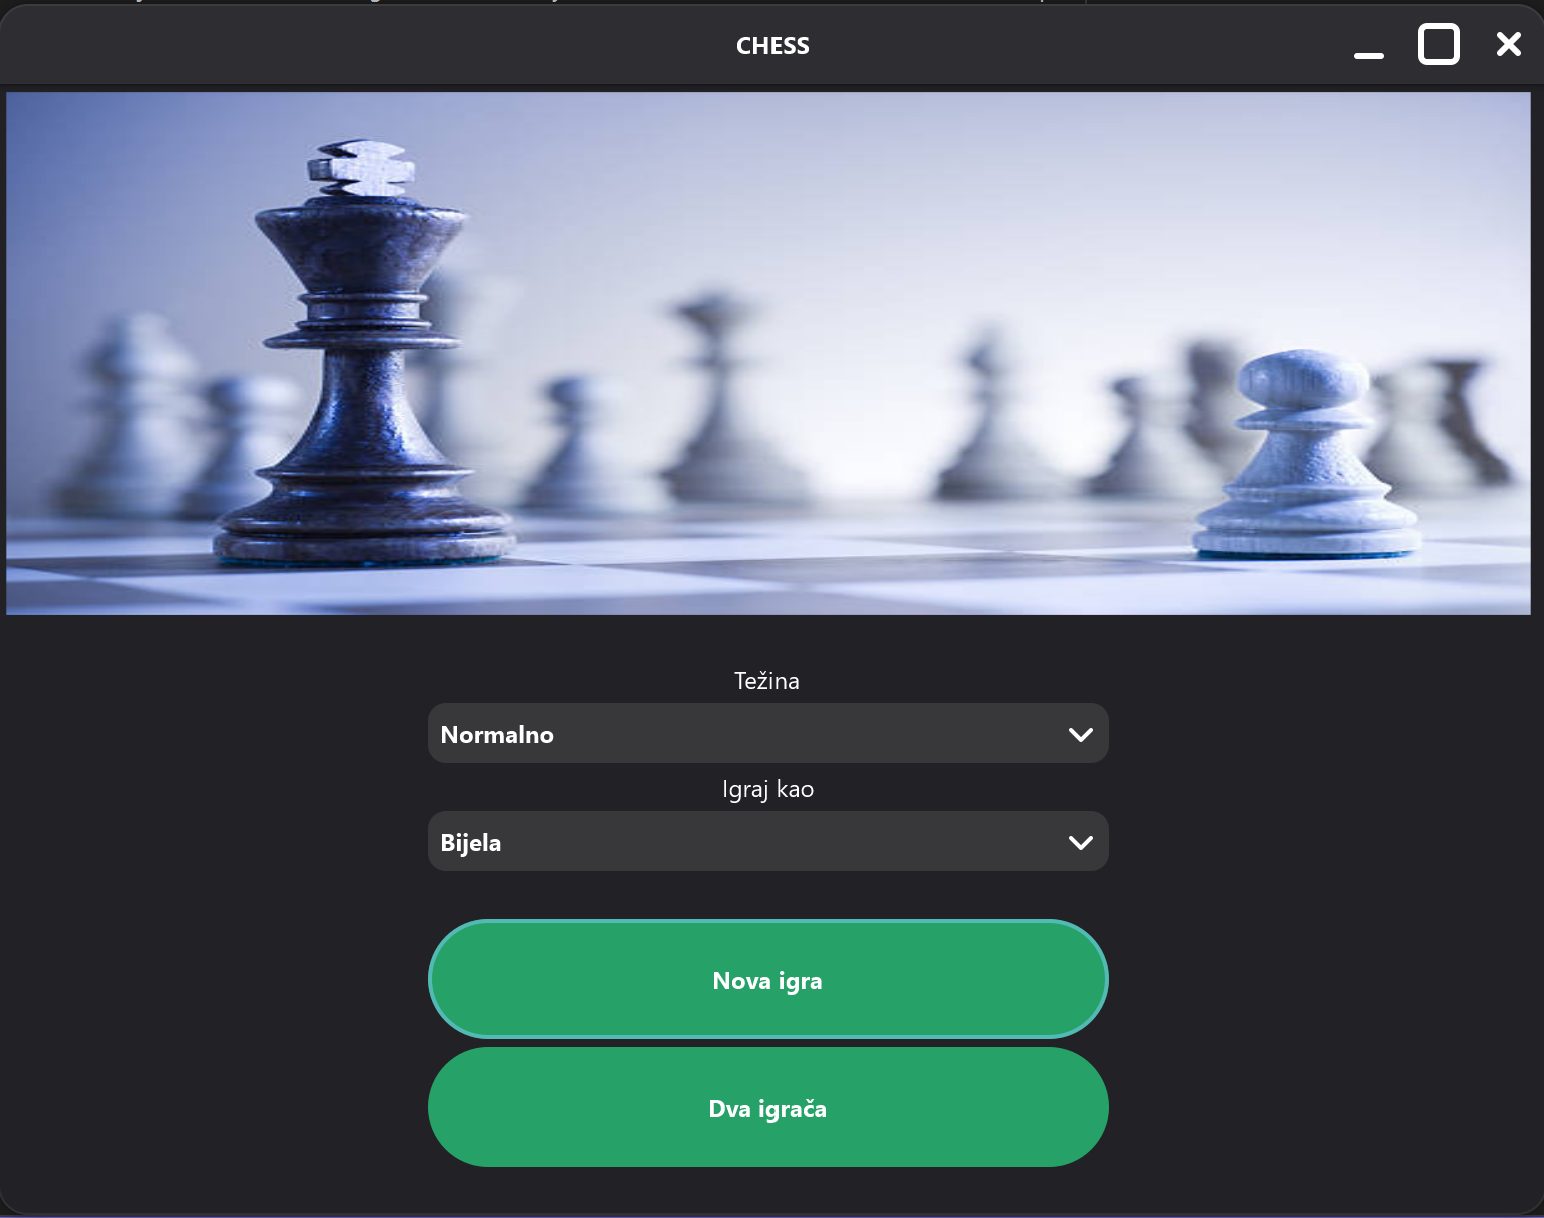
\includegraphics[width=0.62\columnwidth]{Images/start.png}
\caption{Start window (Bosnian interface): difficulty, side selection, new game against the bot or two-player mode.}
\label{fig:start}
\end{figure}

\begin{figure}[t]
\centering
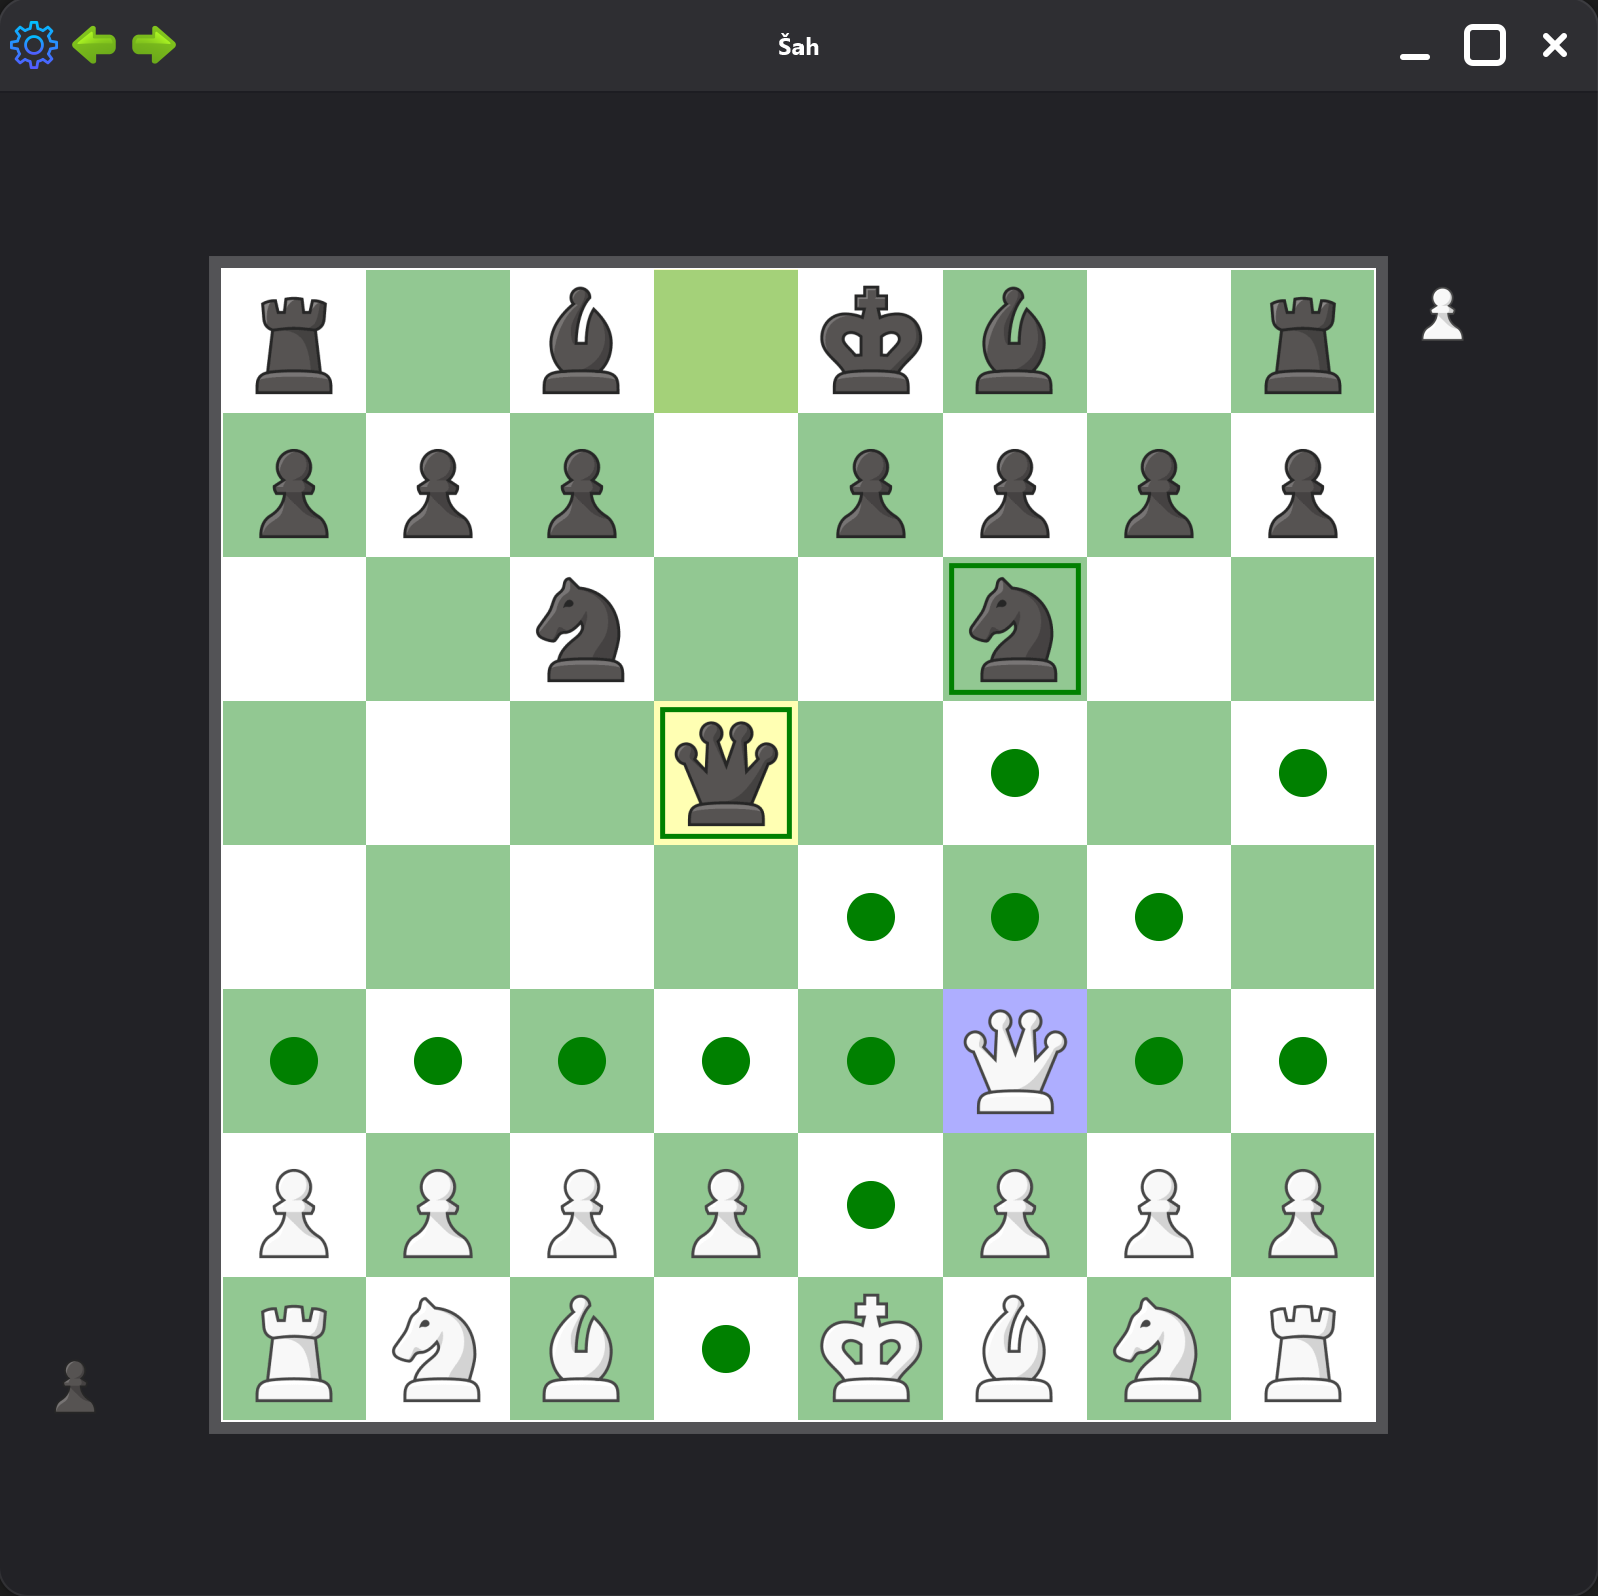
\includegraphics[width=0.8\columnwidth]{Images/board.png}
\caption{Game window: the white queen has been picked up and its legal destinations are marked; the bot's last move (knight to f6) is outlined, captured pieces appear in the side panels, and the toolbar offers settings, undo and redo.}
\label{fig:board}
\end{figure}
\subsection{Game flow}
\texttt{StartWindow} (Fig.~\ref{fig:start}) lets the player choose human-versus-human or human-versus-bot, the bot's colour and the difficulty. \texttt{Chess} owns the \texttt{ChessBoard}, the move history and a redo stack. Captured pieces are derived from the history rather than tracked separately, so undo and redo need no additional bookkeeping: the history is the single source of truth. Against the bot, undo retracts both the bot's reply and the human's move so the human is again to move. Draw detection covers stalemate, the fifty-move rule, threefold repetition (a ring of recent Zobrist hashes) and insufficient material; the window title shows the game status.

\subsection{Threading}
The search runs on a worker thread. \texttt{maybeBotMove} takes a copy of the position under a short lock, releases it, searches on the copy and posts the chosen move back to the main thread through natID's \texttt{MainThreadSharedFunction} callback. This is what keeps the interface responsive: an earlier version held the lock for the whole search, which froze painting for the bot's entire think time and made the human's own move appear only together with the reply. A small minimum think time is padded after fast replies so that a move never appears instantaneously.

\subsection{Board view}
The board and pieces are drawn on a \texttt{gui::Canvas} using natID's \texttt{Shape} and image primitives. Pieces are moved by drag-and-drop; when a piece is picked up its legal destinations are highlighted, with a distinct marker on squares where the move captures (Fig.~\ref{fig:board}). Promotion opens a four-piece picker (queen first). Panels on either side list the captured pieces, heaviest first. The toolbar offers start/stop, undo, redo, reset and settings; the settings popover switches the interface language (Bosnian or English) via natID's translation resources. Images are registered as resources in \texttt{res/main.xml} and referenced by id, so they resolve correctly whether the application is started from the build folder, from a macOS bundle or from Explorer.

\section{Results}
\label{sec:results}
All measurements were made on the engine compiled stand-alone with GCC~13, \texttt{-O2 -std=c++20}, on a single-core Linux machine; the GUI was not involved.

\subsection{Move-generator correctness (perft)}
\label{sec:perft}
Table~\ref{tab:perft} compares the engine's perft counts with the published reference values \cite{cpw} for four standard positions: the initial position, Kiwipete (castling, promotions, en passant, pins), position~3 (an endgame with en passant and rook pins) and position~4 (promotions with check). Every count matches, up to 4.9~million leaves. Throughput is 11--17 million nodes per second (Fig.~\ref{fig:perft}), which is the cost of full legality checking by make/unmake and ray-walking sliders; it is far more than the search needs.

\begin{table}[t]
\caption{Perft node counts versus the published reference values. All entries agree.}
\label{tab:perft}
\centering
\begin{tabular}{@{}lcrrr@{}}
\toprule
Position & Depth & Engine & Reference & Time \\
\midrule
Start position & 4 & 197\,281 & 197\,281 & 0.013 s \\
Start position & 5 & 4\,865\,609 & 4\,865\,609 & 0.288 s \\
Kiwipete & 3 & 97\,862 & 97\,862 & 0.007 s \\
Kiwipete & 4 & 4\,085\,603 & 4\,085\,603 & 0.331 s \\
Position 3 & 5 & 674\,624 & 674\,624 & 0.060 s \\
Position 4 & 4 & 422\,333 & 422\,333 & 0.038 s \\
\bottomrule
\end{tabular}
\end{table}

\begin{figure}[t]
\centering
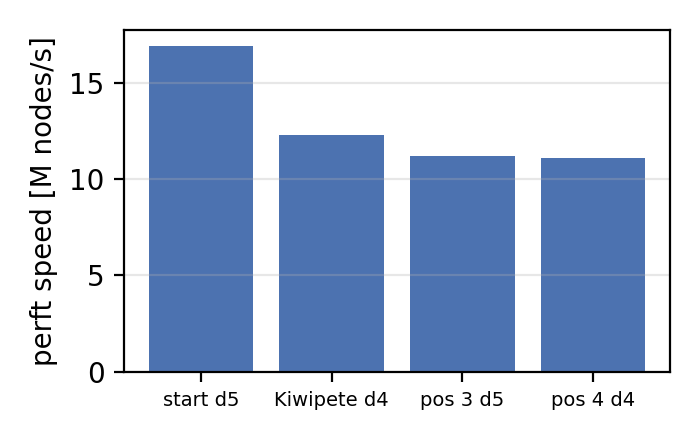
\includegraphics[width=0.75\columnwidth]{Images/perft_speed.png}
\caption{Perft throughput on the four test positions (single core).}
\label{fig:perft}
\end{figure}

\subsection{Search effort}
Table~\ref{tab:search} and Fig.~\ref{fig:scaling} show the number of nodes and the time required to search the start position to a fixed depth, and the Kiwipete middlegame with iterative deepening. The effective branching factor---the ratio of successive node counts---is 3.3 to 6.0 from the start position and 2.1 to 5.1 in Kiwipete, far below the raw branching factor of 20 to 48 legal moves, which quantifies the benefit of alpha--beta together with the ordering heuristics and the transposition table. Depth 6 from the start position takes 0.23~s; the Kiwipete position, with its many captures and long quiescence trees, needs 9.5~s for depth~6, which is why the difficulty levels are expressed in time rather than depth.

\begin{table}[t]
\caption{Search effort by depth (single thread).}
\label{tab:search}
\centering
\begin{tabular}{@{}crrcrr@{}}
\toprule
\multicolumn{3}{c}{Start position, fixed depth} & \multicolumn{3}{c}{Kiwipete, iterative deepening} \\
\cmidrule(r){1-3}\cmidrule(l){4-6}
Depth & Nodes & Time & Depth & Nodes & Time \\
\midrule
2 & 855 & 0.006 s & 3 & 240\,311 & 0.48 s \\
3 & 6\,380 & 0.005 s & 4 & 513\,073 & 0.82 s \\
4 & 21\,429 & 0.009 s & 5 & 2\,614\,022 & 4.42 s \\
5 & 70\,512 & 0.060 s & 6 & 8\,046\,802 & 9.47 s \\
6 & 421\,731 & 0.227 s & & & \\
\bottomrule
\end{tabular}
\end{table}

\begin{figure}[t]
\centering
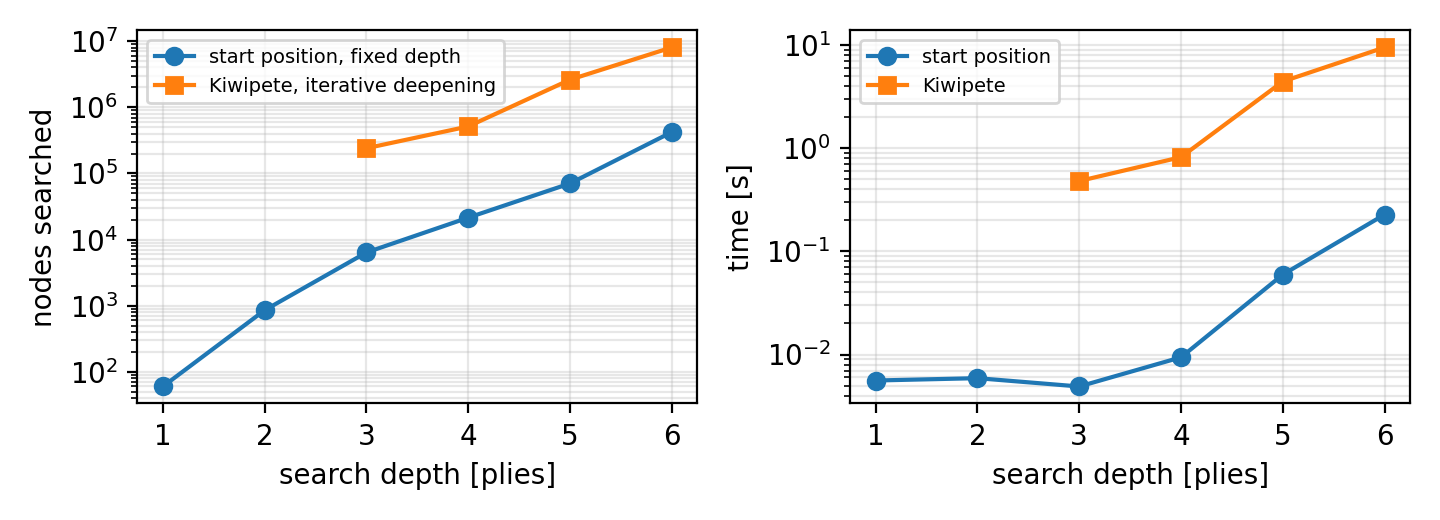
\includegraphics[width=\columnwidth]{Images/search_scaling.png}
\caption{Nodes searched (left) and wall-clock time (right) versus depth; logarithmic vertical axes.}
\label{fig:scaling}
\end{figure}

\subsection{Time-budgeted search}
On the Kiwipete position the timed search reached depth 3 within the 150~ms and 400~ms budgets (42\,491 nodes, 0.09~s), depth 4 within 1~s (240\,311 nodes, 0.47~s) and depth 5 with the 2.2~s Expert budget. On the author's development machine, where the parallel final iteration runs on all cores, the same levels reach one ply deeper in the middlegame and depth~8 in simple endgames, as recorded in the source comments that motivated the budget values.

\subsection{Multithreading}
The root-parallel final iteration could not be measured here because the benchmark machine exposes a single hardware thread; with one worker the parallel and sequential code paths visited the same number of nodes ($\pm0.1\,\%$) in the same time, which at least confirms that the parallel path introduces no overhead when it has nothing to parallelise. Because each thread owns a private transposition table, the expected speed-up on $k$ cores is somewhat below $k$: threads cannot share the transpositions they discover.

\section{Limitations and Future Work}
\textbf{Clock granularity.} The budget is checked only between iterations, and the estimate of the next iteration is based on the previous one. When the branching factor jumps---as it does in Kiwipete between depths 4 and 5, where the cost grows fivefold---the last iteration can overrun the budget: with a 2.5~s budget the search took 4.7~s in this position. A deadline check inside the recursion, aborting the current iteration and keeping the previous best move, would make the response time exact.

\textbf{Shared transposition table.} A lock-free shared table (lazy SMP) would let the worker threads benefit from each other's work and is the standard next step after root splitting.

\textbf{Search extensions.} The engine has no null-move pruning, late-move reductions, check extensions or opening book. Each of these is a well-understood addition that would add one to two plies at the same budget.

\textbf{Evaluation.} The evaluation is hand-tuned; the weights have not been fitted against a reference engine or a game database, and there is no endgame tablebase, so some theoretically drawn endgames are played out to the fifty-move rule.

\section{Conclusion}
The project delivers a complete, verified chess program. The bitboard engine reproduces the published perft counts of four standard positions exactly, which is the strongest available evidence that the rules---including castling, en passant, promotion and pins---are implemented correctly. The opponent applies the classical adversarial-search toolkit in full: negamax with alpha--beta pruning, quiescence, a Zobrist-keyed transposition table, MVV--LVA, killer and history ordering, iterative deepening with a root-parallel final iteration and mate-distance scoring, on top of a seven-term evaluation function. Measured effective branching factors of 2--6 against a raw factor of 20--48 show these techniques doing their job. Defining difficulty as a time budget per move, chosen by measuring the cost of each extra ply, gives a consistent playing experience, and moving the search off the interface thread keeps the natID front end responsive throughout. The engineering lessons that carried the most weight were the two that made errors visible: perft for the move generator and the incrementally maintained hash, whose desynchronisation immediately exposed a move-generation bug.

\begin{thebibliography}{9}
\bibitem{knuth} D. E. Knuth and R. W. Moore, ``An analysis of alpha-beta pruning,'' \emph{Artificial Intelligence}, vol. 6, no. 4, pp. 293--326, 1975.
\bibitem{shannon} C. E. Shannon, ``Programming a computer for playing chess,'' \emph{Philosophical Magazine}, vol. 41, no. 314, pp. 256--275, 1950.
\bibitem{zobrist} A. L. Zobrist, ``A new hashing method with application for game playing,'' Tech. Rep. 88, Computer Sciences Dept., Univ. of Wisconsin, 1970.
\bibitem{cpw} Chess Programming Wiki, ``Perft results'' and ``Bitboards,'' \url{https://www.chessprogramming.org}, accessed Sept. 2026.
\bibitem{russell} S. Russell and P. Norvig, \emph{Artificial Intelligence: A Modern Approach}, 4th ed. Pearson, 2021, ch. 5.
\bibitem{natid} I. D\v{z}afi\'c, \emph{natID framework: Common/Include SDK documentation}, 2026.
\end{thebibliography}

\end{document}
